{\color{PineGreen}\section{Contact Tracing}}

Contact tracing is a strategy for breaking transmission chains and controlling the spread of the disease. Contact tracing is most effective as a means of containing flareups. Applying this strategy can prevent exponential growth in new cases, protect health-care systems and potentially save lives.
\\
{\color{PineGreen}\subsection{Description}}
It involves identifying infected persons, finding those with whom the infected person may have been in close contact while infectious, locating and testing these close contacts. If a close contact is found to be infected, the disease-investigation process starts again.
\\
It is extremely important to identify asymptomatic or paucisymptomatic because these cases can transmit the virus. This investigation helps public-health departments to draw lines of transmission accurately. Contact tracing could help find those people and ask them to self-isolate.\\

{\color{PineGreen}\subsection{Current base approaches}}

The algorithm for the management of contacts of probable or confirmed COVID-19 cases issued by the 
European Center for Disease prevention and control is described below:

\begin{center}
	\begin{figure}[H]
	    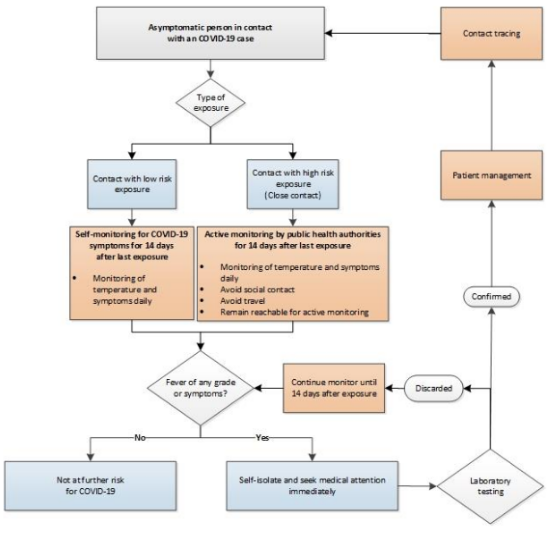
\includegraphics[scale=0.7]{imgs/algo_eu.png}
 		\caption{Algorithm for the management of contacts of probable or confirmed COVID-19}
 		\label{fig:algo_eu}
	\end{figure}
\end{center}

During the contact investigation, the IDD makes a distinction between high-risk and low-risk contacts. 

\begin{center}
	\begin{figure}[H]
	    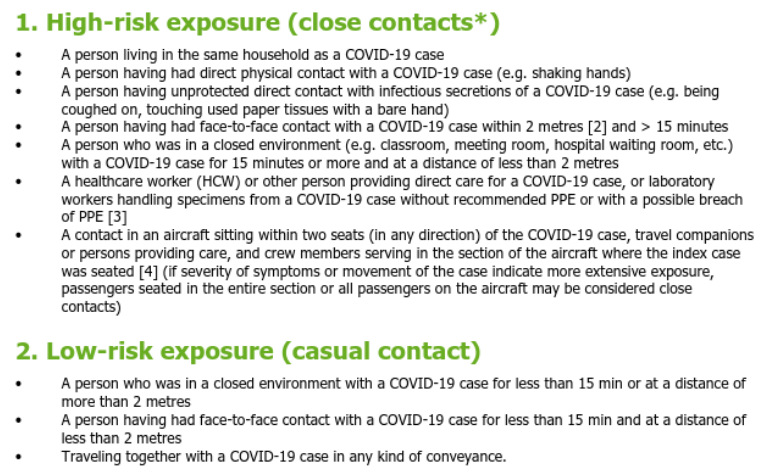
\includegraphics[scale=0.5]{imgs/hi_low.png}
 		\caption{Distinction between high and low-risk contacts}
 		\label{fig:hi_low}
	\end{figure}
\end{center}

Current modes of operation in the Netherlands\cite{bib3} and in Italy are described in the following sub sections.\\
{\color{PineGreen}\subsubsection{The Netherlands}}
If a person tests positive for the coronavirus, the Infectious Disease department (IDD) of the municipal or regional Health Service will be notified. The IDD contacts the patient or another designated contact person and maps out who the patient has been in contact with during the contagious period. From the first day of illness of the patient - the day someone starts to cough or develop symtoms - until the last moment of contact that the patient has had with someone.
\\
{\color{PineGreen}\subsubsection{Italy}}
In Italy, we rely on covid patients' past memories. They ask if they remember who they have been in contact with. If they miss someone, the forgotten citizen will be potentially the next patient 0 and the deadly will loop strike back.
